\newpage

\titleformat % design des titres des chapitres
{\chapter}
[display]
{\centering\normalfont\Large\scshape\bfseries}
{\rule[3pt]{0.15\linewidth}{3pt}\quad\chaptertitlename~\thechapter\quad \rule[3pt] {0.15\linewidth}{3pt}}
{0\baselineskip}%espace vertical entre chapitre et nom du chapitre
{\rule{\linewidth}{0.5pt}\break\Huge}
[\vspace{-0.5\baselineskip}\rule{\linewidth}{0.5pt}\vspace{0\baselineskip}]

\let\clearpage\relax% Stop LaTeX from going to a new page; and
\vspace*{5.5cm}%

\chapter{Etudes des besoins}
Le présent chapitre a pour but de définir les besoins fonctionnels et non
fonctionnels, après avoir décrit les processus métiers, et les règles de gestion.

\newpage

\section{Description du projet}
\subsection{Objectifs fonctionnels du projet}

L’objectif principal du projet est la facilitation de saisie des données ainsi que l’aide à la prise de décision, de passer d’un modèle de travail qui utilisait plusieurs fichier Excel partager avec plusieurs Equipe pour prendre la décision et s’organiser vers un modèle qui est centré sur une seul application Power Apps qui met en relation les différentes entités du system. 
\\

Dans un premier temps, il s’agit de définir de manière claire et précise les besoins et les attentes d’un système d’information permettant d’automatiser les remontées de l’équipe vers différentes entités, ainsi que la saisie des Deals, choix des Squads, l’affectation des ressources et l’affichage des statistiques dans un tableau de bord avec différents filtres. 
\\

Fournir une visibilité sur les prévisions financières au niveau du compte et du portefeuille, y compris les changements de revenus mensuels et trimestriels. Ce système devra être capable de gérer les relations clients, la saisie des différents deals pour assurer un suivi par les Services Lines, un Reporting et un suivi des indicateurs.
\\

Dans un second temps, le développement du système d’information devra permettre de garder la trace de tous les échanges afin de pouvoir établir des statistiques et prendre la décision du gain du deal.
\\

Tout au long du projet, la notion de passage à l’échelle devra être prise en compte. L’objectif à long terme de la conception et du développement d’un tel système d’information est de pouvoir être utilisé par tous les acteurs de l’entreprise.

\subsection{Fonctionnalités ciblées}

Les fonctionnalités attendues de l'application sont les suivantes :
\\

\begin{itemize}
    \item \textbf{Ajout de la masse salariale}
    \item \textbf{Réduction de la masse salariale}
    \item \textbf{Optimisation de la masse salariale}
    \item \textbf{Consultation des soumission de la masse salariale}
    \item \textbf{Ajout d'un nouveau projet au niveau du DCT}
    \item \textbf{Modification d'un projet au niveau du DCT}
    \item \textbf{Fermeture d'un projet au niveau du DCT}
    \item \textbf{Consultation des soumissions au niveau du DCT}
    \item \textbf{Consultation des statistiques et tableau de bord}
\end{itemize}


\section{Contraintes du projet}

\subsection{Contraintes en termes de délais}
A partir de la livraison du cahier des charges, nous disposons d’environ quatre mois pour la réalisation du projet. Le délai semble court mais reste suffisant pour se concentrer sur la partie prévue pour le projet de fin d’études.

\subsection{Contraintes de sécurité}
La gestion de la sécurité est la principale contrainte de notre système. L'application doit posséder une gestion de privilèges et de niveaux d'accès pour les différents types d'utilisateurs (RH, administration, ...). Selon leur statut, le contenu des pages varie et l'accès aux informations avec un statut supérieur est interdit.

\subsection{Contraintes techniques}

Pour le développement de notre système, nous disposons d’une architecture
existante sur laquelle nous devrons baser notre application. La structure de notre système doit être extensible pour la mettre en place facilement dans les autres unités de l’entreprise. De plus, le développement devra suivre toutes les normes techniques pour une meilleure performance, maintenance et facilité de mise à jour.

\section{Etude de l'existant}

Un GRC, acronyme du terme Gestion de la Relation Client, est un logiciel informatique permettant à une entreprise de gérer les relations qu’elle entretient avec ses clients.
\\\\
Le GRC permet à une entreprise d’optimiser les interactions et les relations avec ses clients, ses prospects, ses suspects, ses utilisateurs, ses partenaires, ses employés et ses fournisseurs. Ce suivi et l’établissement de ces relations permettent à l’entreprise de mieux comprendre les attentes de ses partenaires. Cela va aider l’entreprise à gagner de nouveaux clients, à les fidéliser et à améliorer son organisation.
\\\\
Chaque solution GRC est différente et à un but différent. Idéalement, une solution GRC devra être adaptée au type d’organisation, à la taille et au marché de l’entreprise qui l’utilise. Un même GRC peut être utilisé différemment par les collaborateurs d’une même entreprise. Certaines entreprises utilisent plusieurs solutions GRC simultanément afin de mieux convenir aux besoins de chacun de leurs collaborateurs.
\\\\
\newpage
\\\\
La pipe commerciale est toute la procédure pour gagner une opportunité offerte par le marché commençant par les premières intentions jusqu’à la signature du contrat.
\\\\
Aujourd’hui, la circulation de l’information dans une entreprise est devenue une stratégie de communication interne. En effet, lorsqu’elle circule bien, l’information favorise la communication et devient, de ce fait, facteur de cohésion, de motivation, de décision efficace et de créativité.
\\\\
Le présent système n’arrive pas à satisfaire les attentes de ses utilisateurs à cause du traitement et du fonctionnement manuelle de ce dernier.
\\\\
Pour cette raison, Value Attainement tool a été déclaré comme besoin interne par le service Line APPS, permettant les bonnes interprétations des informations, la facilitation de saisie des données ainsi que l’aide à la prise de décision.
\\

Ce workflow représente le processus CRM de la gestion du pipe commercial entre le
responsable et le commercial : 


\begin{figure}[!h]
    \centering
    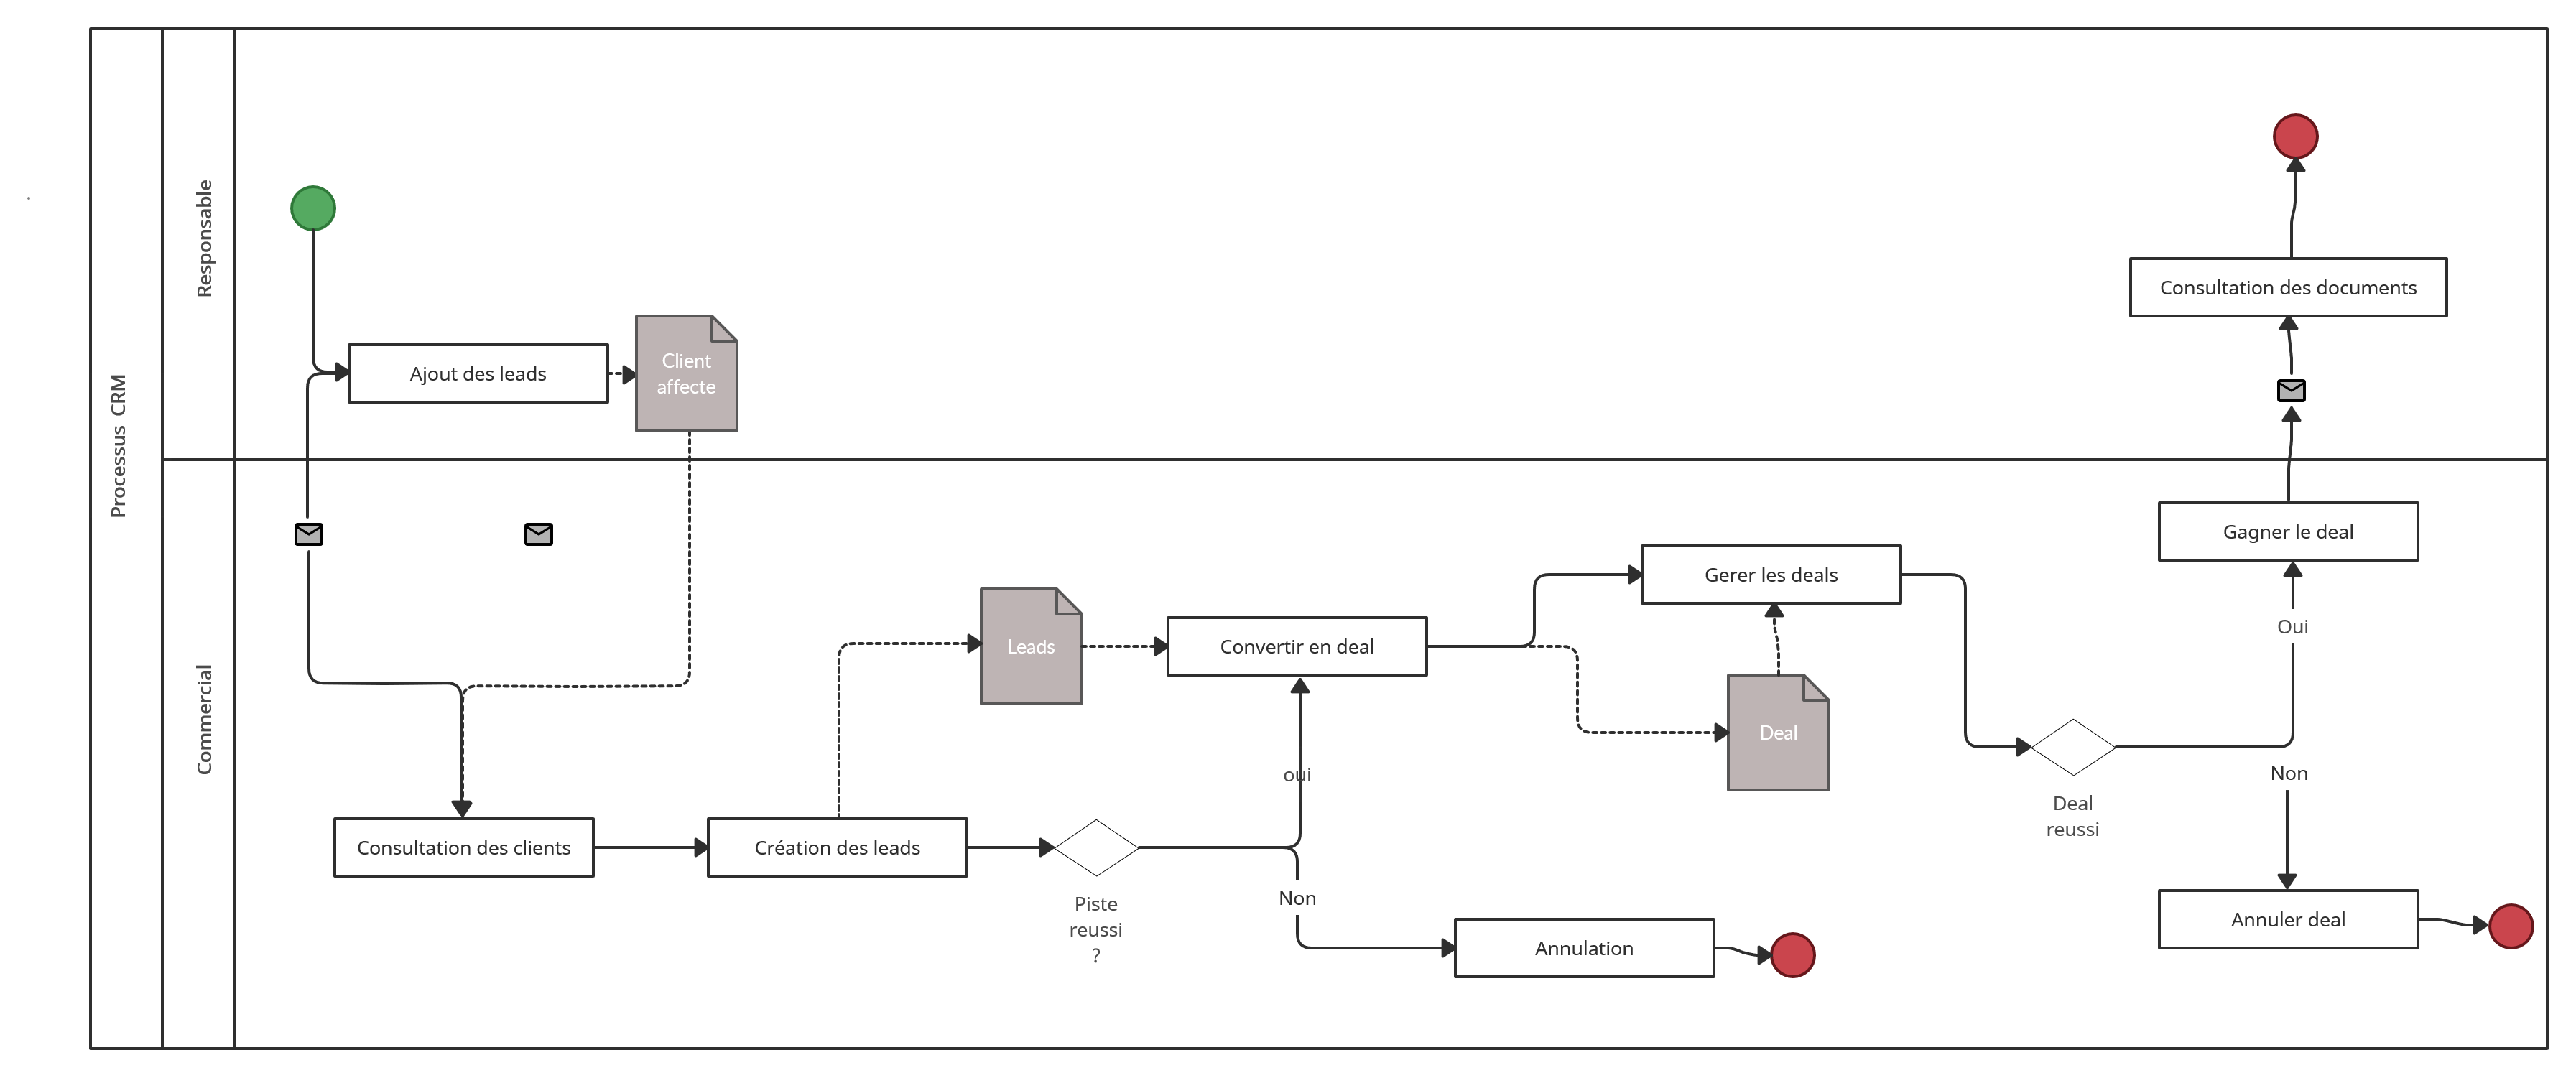
\includegraphics[scale=0.14,keepaspectratio]{Rapport de stage PFE chez DXC/figures/CRM Process.png}
    \caption{Schéma descriptif de la pipe commerciale}
\end{figure}

\newpage
\section{Etude Fonctionnelle}

\subsection{Objectifs fonctionnels}

Pour répondre aux besoins réels et urgents en termes de contraintes fonctionnelles, j'ai travaillé sur ces différents écrans de l'application Value Attainement Tool :
\\
\begin{itemize}
    \item \textbf{Gestion de la masse salariale:} L'application permet à l'utilisateur de gérer sa masse salariale en ajoutant ou bien réduire cette dernière mais aussi l'optimiser.
    \\
    \item \textbf{Consultation des soumission de la masse salariale:} Consulter les différentes soumissions sur la transformation de la masse salariale dans une seul page et aussi la sélection puis la modification possible de chaque soumission.
    \\
    \item \textbf{Gestion de projet DCT:} Ajout d'un nouveau projet DCT, modification de ce dernier et aussi la fermeture du projet.
    \\
    \item \textbf{Consultation des soumissions au niveau du DCT:} Consulter les différentes soumissions.
    \\
    \item \textbf{Consultation des statistiques et tableau de bord:} Accéder à un tableau de bord reliant tous les statistiques importantes au vu d'un deal avec plusieurs filtres tout cela dans une seule page
\end{itemize}

\subsection{Besoins fonctionnels : Fonctionnalités}

\textbf{\color{red}Bloc fonctionnel : Gestion de la masse salariale}
    
Ce bloc fonctionnel est composé de trois écran ou bien page et il permet la gestion de la masse salariale:
\\
\begin{itemize}
    \item L'ajout d'une nouvelle demande pour l'augmentation de la masse salariale 
    \item L'ajout d'une nouvelle demande pour l'Optimisation de la masse salariale 
    \item L'ajout d'une nouvelle demande pour la réduction de la masse salariale 
\end{itemize}

\vspace{0.5cm}
\textbf{\color{red}Bloc fonctionnel : Consultation les soumission de la masse salariale:}
    
Ce bloc fonctionnel est composé d'un seul ecrant qui relie les differentes soumissions de la masse salariale:
\\
\begin{itemize}
    \item La consulation des soumission de la masse salariale
    \item La modification d'une soumission aprés sélection
    \item La modification d'un groupe de soumission
\end{itemize}

\newpage
\textbf{\color{red}Bloc fonctionnel : Gestion de projet DCT}
    
Ce bloc fonctionnel est composé de trois ecran et il permet la gestion des projet DCT: 
\\
\begin{itemize}
    \item L'ajout d'un nouveau projet DCT.
    \item La modification d'un projet DCT.
    \item La fermeture d'un projet DCT.
\end{itemize}

\vspace{0.5cm}
\textbf{\color{red}Bloc fonctionnel : Consultation des soumissions au niveau du DCT}
    
Ce bloc fonctionnel est composé d'un seul ecran qui relie les differentes soumissions des projets DCT.
\begin{itemize}
    \item La consultation des differentes soumission pour projet DCT.
\end{itemize}

\vspace{0.5cm}
\textbf{\color{red}Bloc fonctionnel : Consultation des statistiques et tableau de bord}
    
Ce bloc fonctionnel est composé d'un seul ecran qui relie les differentes soumissions des projets DCT.
\begin{itemize}
    \item L’affichage des statistiques des deals.
\end{itemize}

\subsection{Besoins non fonctionnels}

Pour la bonne gestion d'un grand projet informatique on doit prendre en compte plusieurs éléments importants comme les caractéristiques de qualités qui sont la plupart du temps des besoins implicites.
\\\\
C'est pour cela que nous avons fixé un ensemble d'objectif en termes de qualité auxquels le système doit répondre autant que possible, ces différents objectifs sont :
\\
\begin{itemize}
    \item \textbf{Fiabilité:} Le système doit fonctionner sans défaillance.
    \item \textbf{Disponibilité:} Le système doit être toujours à la disposition des utilisateurs.
    \item \textbf{Réutilisabilité:} Il doit être possible de réutiliser certains modules du
système.
    \item \textbf{Convivialité:} Le système doit être compréhensible, documenté, et son
utilisation doit être facile.
\end{itemize}

\subsection{Acteurs}
Il s’agit de quatre acteurs principaux agissant dans le système :
\\
\begin{itemize}
    \item \textbf{BizDev:} Saisie et évolution du pipe (Deals / calcul des Revenue Mensuels
et TCV…)
    \item \textbf{Service Lines:} Compléter les données relatives aux ressources du deal (HC à facturer / HC à recruter)
    \item \textbf{Réutilisabilité:} Il doit être possible de réutiliser certains modules du
système.
    \item \textbf{Ressource Humaine:} Compléter la donnée relative aux ressources (Starting Date / Hiring
Date)
    \item \textbf{Finance:} Confirmer la données et verifier les budgets.
\end{itemize}


\section{Conclusion}

Dans ce chapitre j’ai donné une description du projet avec ces but et fonctionalités ciblées, les differentes contraites du projet ensuite j'ai présenté l’étude de l’existant, et les besoins fonctionnelles et non fonctionnelles du projet. 
\\
Le chapitre suivant se concentrera sur l’étude technique du projet.

